\section{Experimental Results}
\label{sec:experimental_results}

This section reports the experimental results for the AE, VAE, and CVAE models on the completed Gen-MOR 50K experiment. The dataset contains $50{,}000$ MORNP-style plan vectors with $20$ objective dimensions and a selected MORNP subset of $k=12$ objectives. The evaluation in this section focuses on dataset visualization, model training behavior, latent-space structure, and test-set reconstruction and classification performance. Dominance-validity results are analyzed separately in Section~\ref{sec:dominance_validity_analysis}.

\subsection{Dataset Visualization}
\label{subsec:dataset_visualization}

Before training the generative models, the dataset is visualized to inspect the structure of the objective-vector space. Since each plan vector has $20$ objective dimensions, principal component analysis (PCA) is used to project the vectors into two dimensions for visualization. Let $\operatorname{PCA}_2(\cdot)$ denote the two-dimensional PCA projection. For each objective vector $\mathbf{x}_i$, the visualization point is computed as
\begin{equation}
    \mathbf{u}_i
    =
    \operatorname{PCA}_2(\mathbf{x}_i),
    \qquad
    \mathbf{u}_i \in \mathbb{R}^{2}.
    \label{eq:pca_projection_raw}
\end{equation}

The PCA plot is used to visually compare the distribution of $P^{+}$ and $P^{-}$ samples. In the 50K dataset, the first two principal components explain only a limited portion of the total variance, so the PCA plot should be interpreted as an exploratory low-dimensional projection rather than a complete description of the dominance structure. The plot shows that the two classes overlap in the first two principal components, indicating that the learned models must capture structure beyond what is visible in a simple two-dimensional PCA view.

\begin{figure}[H]
    \centering
    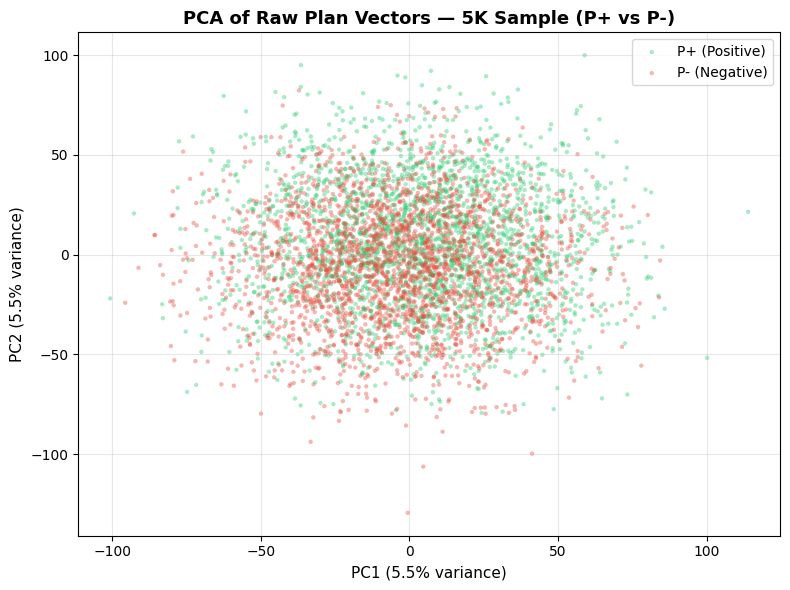
\includegraphics[width=0.78\textwidth]{figures/05_pca_raw.png}
    \caption{PCA visualization of the raw Gen-MOR 50K objective vectors. Points are colored by dominance label, where $P^{+}$ denotes nondominated plans and $P^{-}$ denotes dominated plans.}
    \label{fig:raw_dataset_pca}
\end{figure}

The PCA visualization in Fig.~\ref{fig:raw_dataset_pca} does not define dominance validity, but it helps illustrate the difficulty of the learning problem. Since the classes are not perfectly separated in the first two principal components, reconstruction and classification metrics must be interpreted together with dominance-specific validation.

\subsection{Class Distribution Results}
\label{subsec:class_distribution_results}

The final dataset is near-balanced, containing $25{,}209$ $P^{+}$ plans and $24{,}791$ $P^{-}$ plans. This near balance prevents the classifier from achieving high accuracy simply by favoring one majority class. The distribution is summarized in Table~\ref{tab:result_class_distribution}.

\begin{table}[H]
\centering
\caption{Class distribution used in the Gen-MOR 50K experiment.}
\label{tab:result_class_distribution}
\begin{tabular}{lccc}
\hline
\textbf{Class} & \textbf{Symbol} & \textbf{Label} & \textbf{Count} \\
\hline
Nondominated plans & $P^{+}$ & $1$ & $25{,}209$ \\
Dominated plans & $P^{-}$ & $0$ & $24{,}791$ \\
\hline
Total & -- & -- & $50{,}000$ \\
\hline
\end{tabular}
\end{table}

\begin{figure}[H]
    \centering
    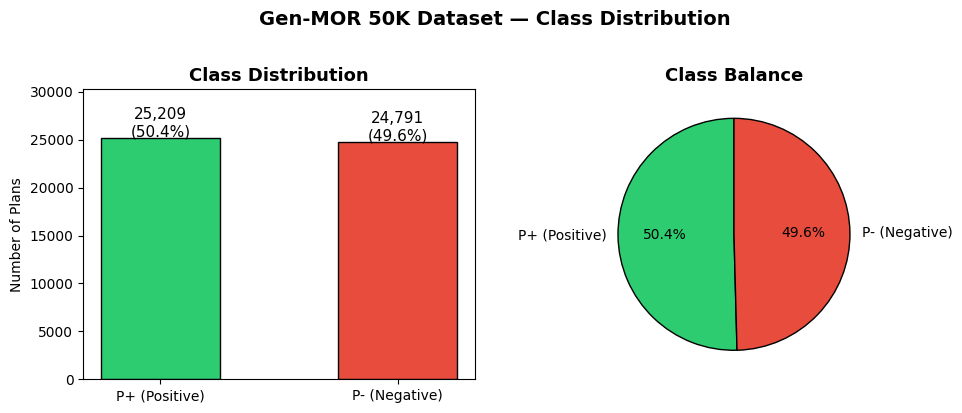
\includegraphics[width=0.80\textwidth]{figures/01_class_distribution.png}
    \caption{Class distribution of the Gen-MOR 50K dataset. The dataset is near-balanced, with $50.4\%$ $P^{+}$ plans and $49.6\%$ $P^{-}$ plans.}
    \label{fig:class_distribution}
\end{figure}

The near-balanced class distribution shown in Fig.~\ref{fig:class_distribution} makes classification metrics easier to interpret and provides comparable representation for both conditional generation targets in the CVAE.

\subsection{Autoencoder Training Results}
\label{subsec:ae_training_results}

The AE model is evaluated using total loss, reconstruction loss, and classification loss. The total loss follows Eq.~\eqref{eq:ae_total_loss}. During training, the reconstruction loss measures how well the decoder recovers objective vectors from the latent representation, while the classification loss measures how well the latent representation supports separation between $P^{+}$ and $P^{-}$.

\begin{figure}[H]
    \centering
    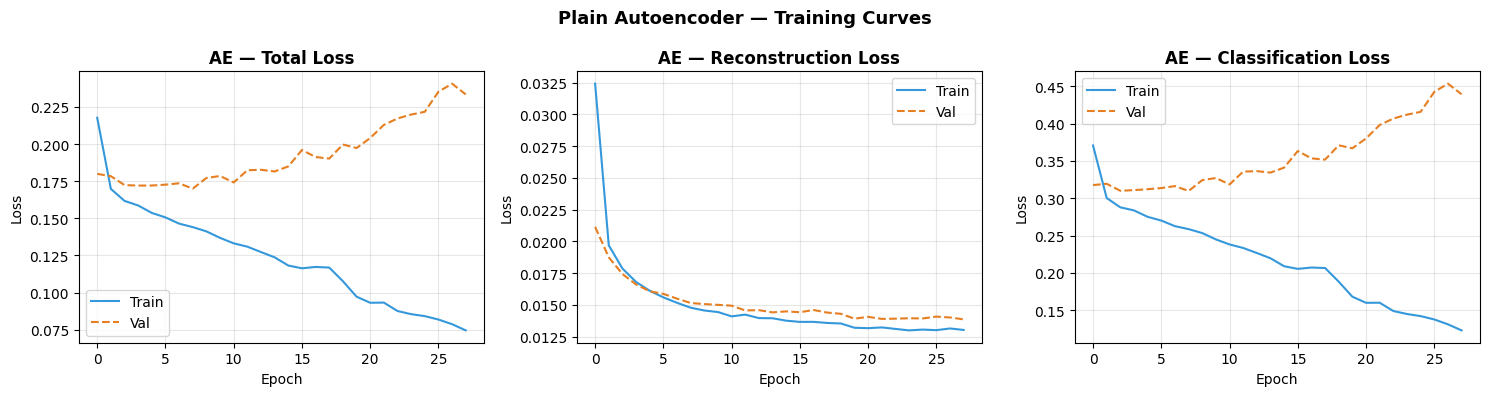
\includegraphics[width=1.0\textwidth]{figures/06_ae_loss_curves.png}
    \caption{AE training curves showing total loss, reconstruction loss, and classification loss over epochs.}
    \label{fig:ae_training_loss}
\end{figure}

The AE trained for $28$ epochs before early stopping. On the test set, it achieved a reconstruction MSE of $0.0150$, classification accuracy of $85.8\%$, and weighted F1 score of $0.8584$. These results show that the deterministic autoencoder learns a useful compressed representation for reconstructing MORNP-style objective vectors and predicting dominance labels.

\subsection{VAE Training Results}
\label{subsec:vae_training_results}

The VAE model is evaluated using total loss, reconstruction loss, KL divergence, and classification loss. The total loss follows Eq.~\eqref{eq:vae_total_loss}. Unlike the AE, the VAE must balance reconstruction quality with latent-space regularization. Therefore, the KL-divergence curve is an important part of the training analysis.

\begin{figure}[H]
    \centering
    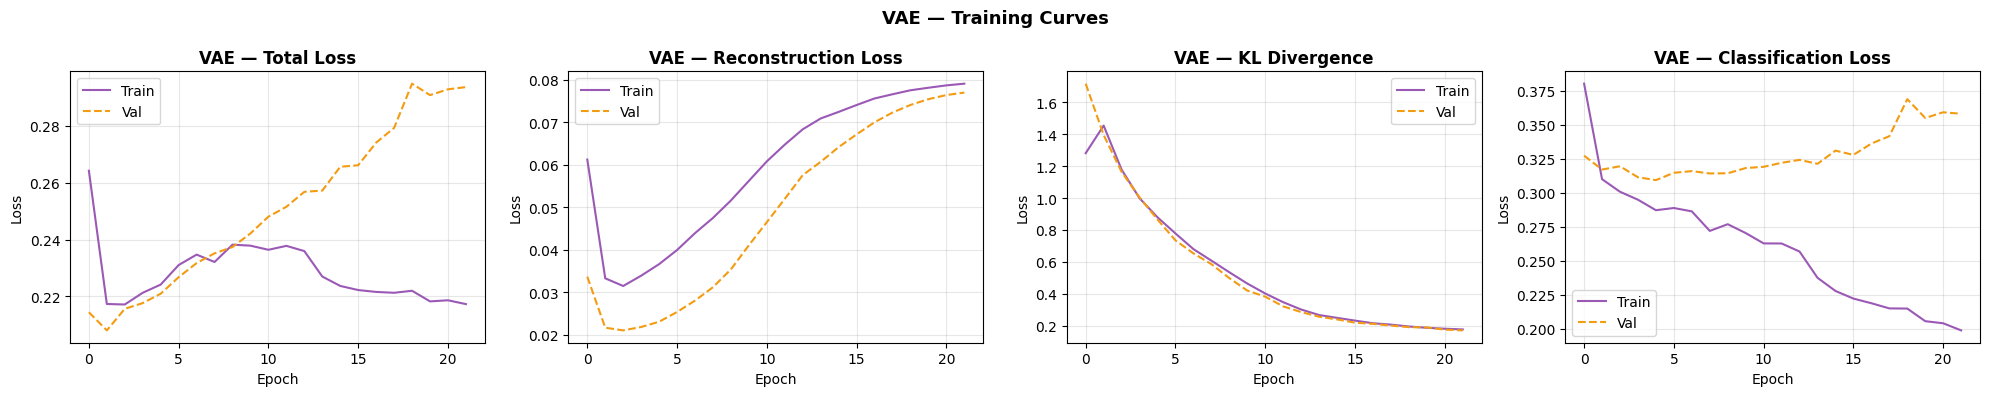
\includegraphics[width=1.0\textwidth]{figures/08_vae_loss_curves.png}
    \caption{VAE training curves showing total loss, reconstruction loss, KL divergence, and classification loss over epochs.}
    \label{fig:vae_training_loss}
\end{figure}

The VAE trained for $22$ epochs before early stopping. On the test set, it achieved a reconstruction MSE of $0.0215$, classification accuracy of $85.4\%$, and weighted F1 score of $0.8537$. Compared with the AE, the VAE has slightly higher reconstruction error, which is expected because the latent space is regularized for sampling. However, its classification performance remains close to that of the AE, indicating that the probabilistic latent representation still captures useful class-relevant structure.

\subsection{CVAE Training Results}
\label{subsec:cvae_training_results}

The CVAE model is evaluated using total loss, reconstruction loss, KL divergence, and classification loss. The total loss follows Eq.~\eqref{eq:cvae_total_loss}. The main difference between the CVAE and VAE is that the CVAE receives the dominance label as a conditioning input. This makes it possible to generate samples intended for a specific class, as shown in Eq.~\eqref{eq:cvae_positive_generation} and Eq.~\eqref{eq:cvae_negative_generation}.

\begin{figure}[H]
    \centering
    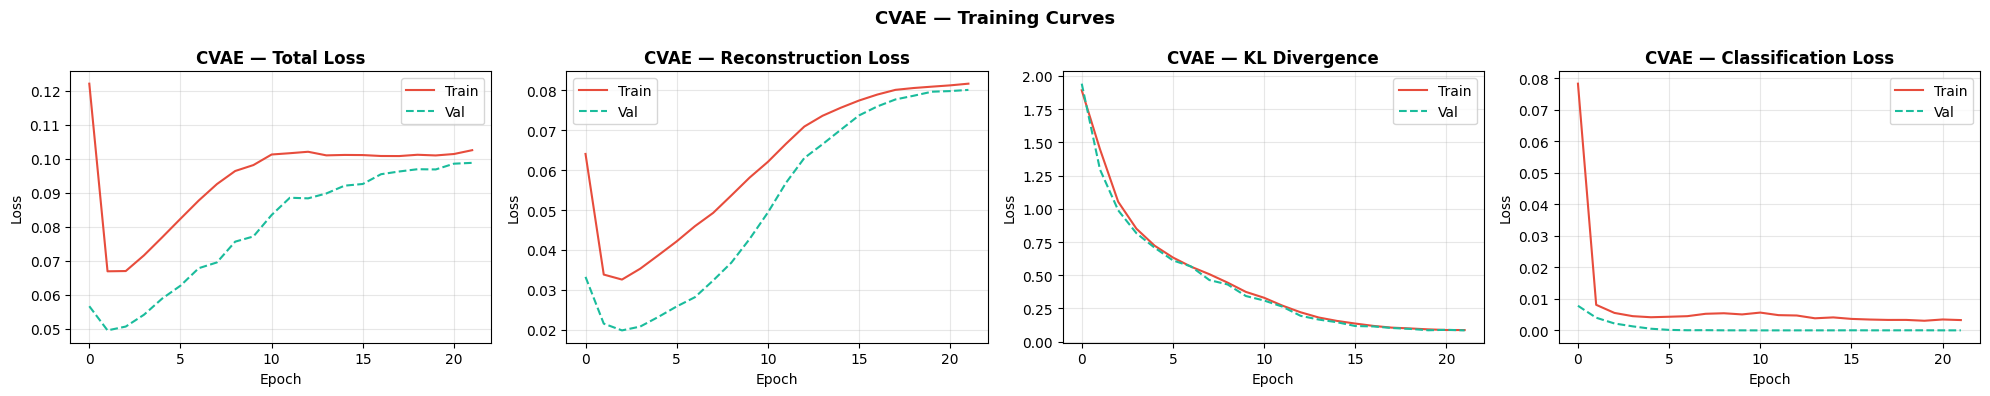
\includegraphics[width=1.0\textwidth]{figures/10_cvae_loss_curves.png}
    \caption{CVAE training curves showing total loss, reconstruction loss, KL divergence, and classification loss over epochs.}
    \label{fig:cvae_training_loss}
\end{figure}

The CVAE trained for $22$ epochs before early stopping. On the test set, it achieved a reconstruction MSE of $0.0213$, classification accuracy of $67.4\%$, and weighted F1 score of $0.6741$. The reconstruction error is close to the VAE result, but the classification score is lower. This suggests that while the CVAE can reconstruct objective vectors and enables class-conditioned generation, its learned latent representation is less effective for separating $P^{+}$ and $P^{-}$ in this experiment.

\subsection{Latent Space Analysis}
\label{subsec:latent_space_analysis}

Latent-space analysis is used to inspect whether the models learn representations that preserve class structure. For each trained model, latent representations are extracted and projected into two dimensions using PCA:
\begin{equation}
    \mathbf{v}_i
    =
    \operatorname{PCA}_2(\mathbf{z}_i),
    \qquad
    \mathbf{v}_i \in \mathbb{R}^{2}.
    \label{eq:latent_pca_projection}
\end{equation}

\begin{figure}[H]
    \centering
    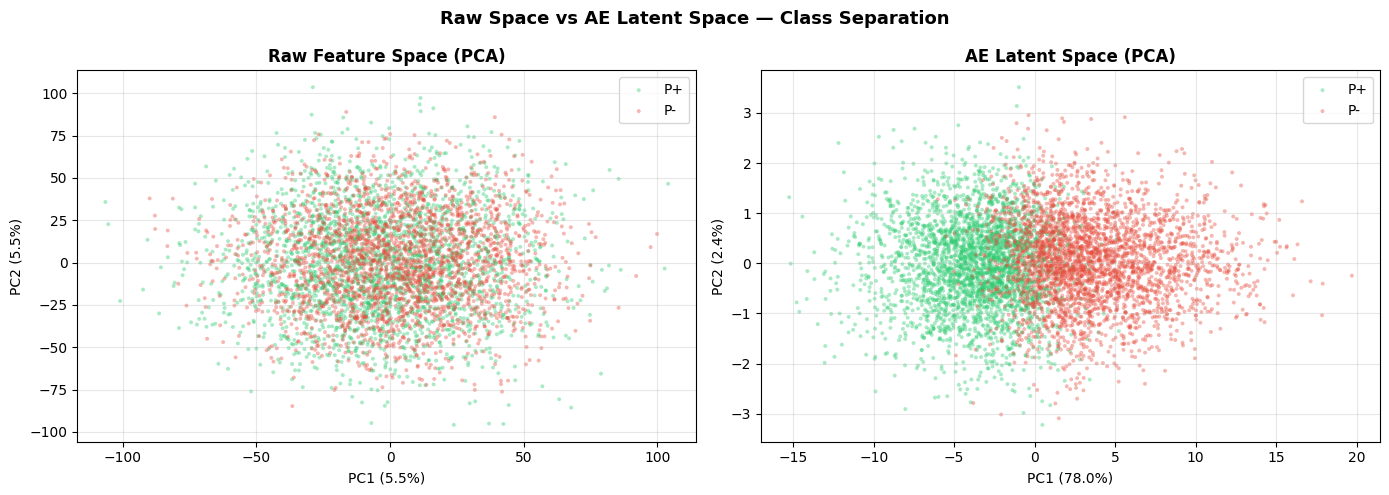
\includegraphics[width=0.90\textwidth]{figures/07_ae_latent_space.png}
    \caption{PCA visualization comparing the raw feature space and the AE latent space. Points are colored by $P^{+}$ and $P^{-}$ labels.}
    \label{fig:latent_space_pca}
\end{figure}

If the latent PCA plot shows stronger class organization than the raw PCA plot, this suggests that the model has learned a representation that captures dominance-relevant information. However, latent separation alone is not enough to prove dominance-preserving generation. Generated samples must still be checked using DVR.

\subsection{Reconstruction and Classification Comparison}
\label{subsec:reconstruction_classification_comparison}

The final reconstruction and classification results are compared across AE, VAE, and CVAE in Table~\ref{tab:model_performance_comparison}. These values are computed on the held-out test set of $7{,}500$ plans.

\begin{table}[H]
\centering
\caption{Reconstruction and classification comparison across Gen-MOR models on the 50K dataset.}
\label{tab:model_performance_comparison}
\begin{tabular}{|l|c|c|c|}
\hline
\textbf{Model} & \textbf{MSE} & \textbf{Accuracy} & \textbf{Weighted F1 Score} \\
\hline
AE & $0.0150$ & $85.8\%$ & $0.8584$ \\
VAE & $0.0215$ & $85.4\%$ & $0.8537$ \\
CVAE & $0.0213$ & $67.4\%$ & $0.6741$ \\
\hline
\end{tabular}
\end{table}

The AE achieves the lowest reconstruction error and the highest classification performance among the three models. The VAE performs slightly worse in reconstruction but remains close to the AE in classification, while also supporting latent-space generation. The CVAE provides class-conditioned generation, but its lower classification performance suggests that conditioning alone does not guarantee stronger class separation. More importantly, the best model under standard reconstruction and classification metrics is not necessarily the best model for dominance-preserving generation. Therefore, the next section evaluates generated samples using DVR.